%\renewcommand\chaptername{Mission de stage}
\titleformat{\chapter}[display]
  {\normalfont\bfseries}{}{0pt}{\Large}

\chapter{Mission de stage}

Dans cette section, je vais décrire la mission du stage plus en détails. Je vais parler de la problématique et des besoins tout en les comparant à des solutions déjà existantes. Ensuite, je vais traiter comment j'ai répondu au problème et avec quels outils. Je vais détailler les différents acteurs en relation avec l'application et leur point de vue par rapport à son utilisation. Enfin, je vais parler des différentes étapes de réalisation.\\

\section{Problématique}

\subsection{Contexte : C.A.T.}

C.A.T., ou "Correcteur Automatique à base de Tests", est une plate-forme développée par M. Delbot et un groupe d'étudiant permettant aux professeurs de communiquer des exercices à leurs élèves qui en retour répondent à ses exercices en répondant directement sur la plate-forme qui s'occupe de "corriger" leurs travaux.\\

C.A.T. est basé sur une application nommée "La Moulinette" développée un an auparavant en tant que première version qui permettait déjà de communiquer et de corriger des exercices. Elle était cependant trop fragile pour accueillir un plus grand nombre d'utilisateurs et était ciblé pour un groupe en particulier. Après une revue, il a été décidé de refaire l'application avec des bases plus solides et un déploiement plus large sous la forme de C.A.T.\\

Cette plate-forme réalisée sous Django/Python est équipé d'une API en Python et en C++ utilisant la bibliothèque clang qui peut déjà lire les travaux rendues et d'effectuer une analyse de la validité par rapport aux normes de C ainsi que les règles imposés par l'exercice.\\

\subsection{Problématique}

Cette API en revanche n'agit que sur des fichiers en C, et la plate-forme veut avancer sur de multiples types de fichiers. Parmi ces fichiers en vue, l'HTML, le SQL et le PHP qui sont enseignés en bas niveau chez les licences pour qui la plate-forme a été réalisé dans un premier temps.\\

\begin{center}
Réaliser un outil permettant de lire des fichiers HTML/SQL/PHP, de générer des tests et de les exécuter sur ces nouveaux types de fichiers pour l'intégrer, avec l’outil précédent, à la plate-forme C.A.T.
\end{center}

\subsection{Les besoins}

Nous avons donc besoin d'une API qui permettra, comme l'outil précédent de lire dans les fichier HTML, SQL et PHP, de générer les tests à partir de l'analyse et les exécuter sur des fichiers de même type.\\

Il faudra que cette outil soit intégrable dans la plate-forme C.A.T. et qu'il soit utilisable de la même manière ou proche que l'outil déjà existant sur la plate-forme.\\

Comme pour l'outil précédent, il faudra un moyen de pouvoir lire dans les fichiers ciblés et d'extraire les informations nécessaires à la génération et à l’exécution des tests.\\

Pour cela, j'ai divisé l'outil en deux : le parser et l'API. Le parser se charge d'extraire les informations nécessaires et les stocker. L'API s'en servira pour récupérer les informations nécessaires à l'analyse des fichiers qu'il lui fournira afin de générer et exécuter les tests à effectuer.\\

Enfin, il faudra écrire les tests qui seront à générer, en gardant un esprit critique et un point de vue éducatif puisqu'il s'agit de tests qui serviront à corriger le produit d'utilisateurs qui ont un bas niveau.\\

\subsection{L'existant}

Dans un cadre éducatif, il n'existe pas réellement de générateur de tests en python pour l'HTML, le SQL et le PHP. Cette API visant à générer les tests à partir d'un fichier, on peut s'inspirer de l'outil déjà réalisé et d'en appliquer sa philosophie dans la nouvelle.\\

Cette API a été réalisé pour la v1 de la plate-forme, la Moulinette. Elle est écrite en deux parties qui communiquent entre elles en s'envoyant des tables en JSON, "JavaScript Object Notation". Il y a une partie écrite en C++/clang, qui sert à extraire les informations de fichiers source C et qui renvoie à deuxième partie le résultat de cette extraction en JSON. Cette deuxième partie est réalisée en Python et s'occupe de l'analyse de ces résultats et de la génération des tests.\\

\section{L'API}

Il m'a été donné comme mission de réaliser une API en Python 3.X en utilisant des librairies Python pour parser les fichiers, les parcourir et générer les tests en fonction de l'analyse.\\

La mission a été divisé en trois grand objectifs a réaliser :\\

\begin{enumerate}
\item génération des tests pour l'HTML
\item pour le SQL
\item pour le PHP
\end{enumerate}

Il a d'abord été réalisé la partie HTML de la génération de tests.\\

\subsection{Les outils de développement}

Le Python est un langage de programmation objet et multi-plate-formes. Grâce à des bibliothèques spécialisées, il peut s'adapter à tout type d'utilisation, d'où son utilisation pour extraire les fichiers dans notre cas. Le Python est l'un des meilleurs langages pour parser certains types de fichiers comme l'HTML. Il a en plus une communauté très fervente qui développe des librairies à des utilisations divers et variés dont un parser SQL nommés sqlparse que j'envisage utilise pour le second objectif de cette mission. Enfin, C.A.T. ayant été réalisé sous Python/Django, cela rend son intégration plus facile.\\

Plusieurs librairies existent pour parser l'HTML, parmi elles se trouve notamment BeautifulSoup et HTMLParser.\\

BeautifulSoup est une librairie d'extraction de fichier HTML et XML tiers. Il permet d'extraire précisément des données contenu dans ce type de fichier très facilement. Il est très populaire parmi les autres parser grâce à sa capacité à extraire des données dans des fichiers complexes et chaotiques. HtmlParser est une librairie intégré qui permet de parcourir de l'HTML et d'en extraire des données comme les balises, le contenu ou les attributs dans ces balises.\\

Après une première comparaison des deux librairies, j'ai opté pour HTMLParser. HTMLParser est une librairie intégré à Python, ce qui veut dire qu'au contraire de BeautifulSoup, il n'y aura pas de module complémentaire à installer à l'intégration de cet objectif de la mission. De plus, dans un cadre éducatif où les fichiers à parser sont relativement simple, BeautifulSoup est plus lourd que ce dont il y a besoin pour l'API. Cependant la possibilité de convertir vers BeautifulSoup reste présente selon la complexité vers laquelle le projet s'oriente.\\

\subsection{Utilisation}

Un travail d'intégration est encore à réaliser afin de comprendre comment l'API fonctionnera sur la plateforme C.A.T., en revanche, dans la version en cours, l'API s'utilise à la ligne de commande.\\

Comme présenté dans ce rapport, les différentes étapes de l'exécution se déroule ainsi :\\

L'utilisateur va en premier lieu fournir un fichier que l'on va appeler "Origine". On considère que ce fichier est sans erreur. L'API va, à l'aide du parser, extraire les balises entrantes, leurs contenus ainsi que leurs attributs. Après avoir extrait les données de ce fichier, l'API va parcourir celle-ci. Lorsqu'elle rencontre une certaine balise, elle va activer la génération de test sur ce type de balise.\\

Une fois cette première analyse réalisée, elle va commencer à générer un script qui va envoyé les données qui va lui servir de comparatif, comme le contenu de la balise "TITRE" par exemple en écrivant un fichier en Python. Elle va, selon les balises qu'elle a rencontré, écrire dans le fichier quels tests sont à réaliser.\\

On exécute ensuite ce script sur un fichier "cible" qui va le parser, en extraire les données, réaliser les tests générer, comparé le contenu à ce qui est attendu et renvoyer un journal citant les différentes étapes qui ont été conclus avec succès ou non.\\

\begin{figure}[ht]
\centering
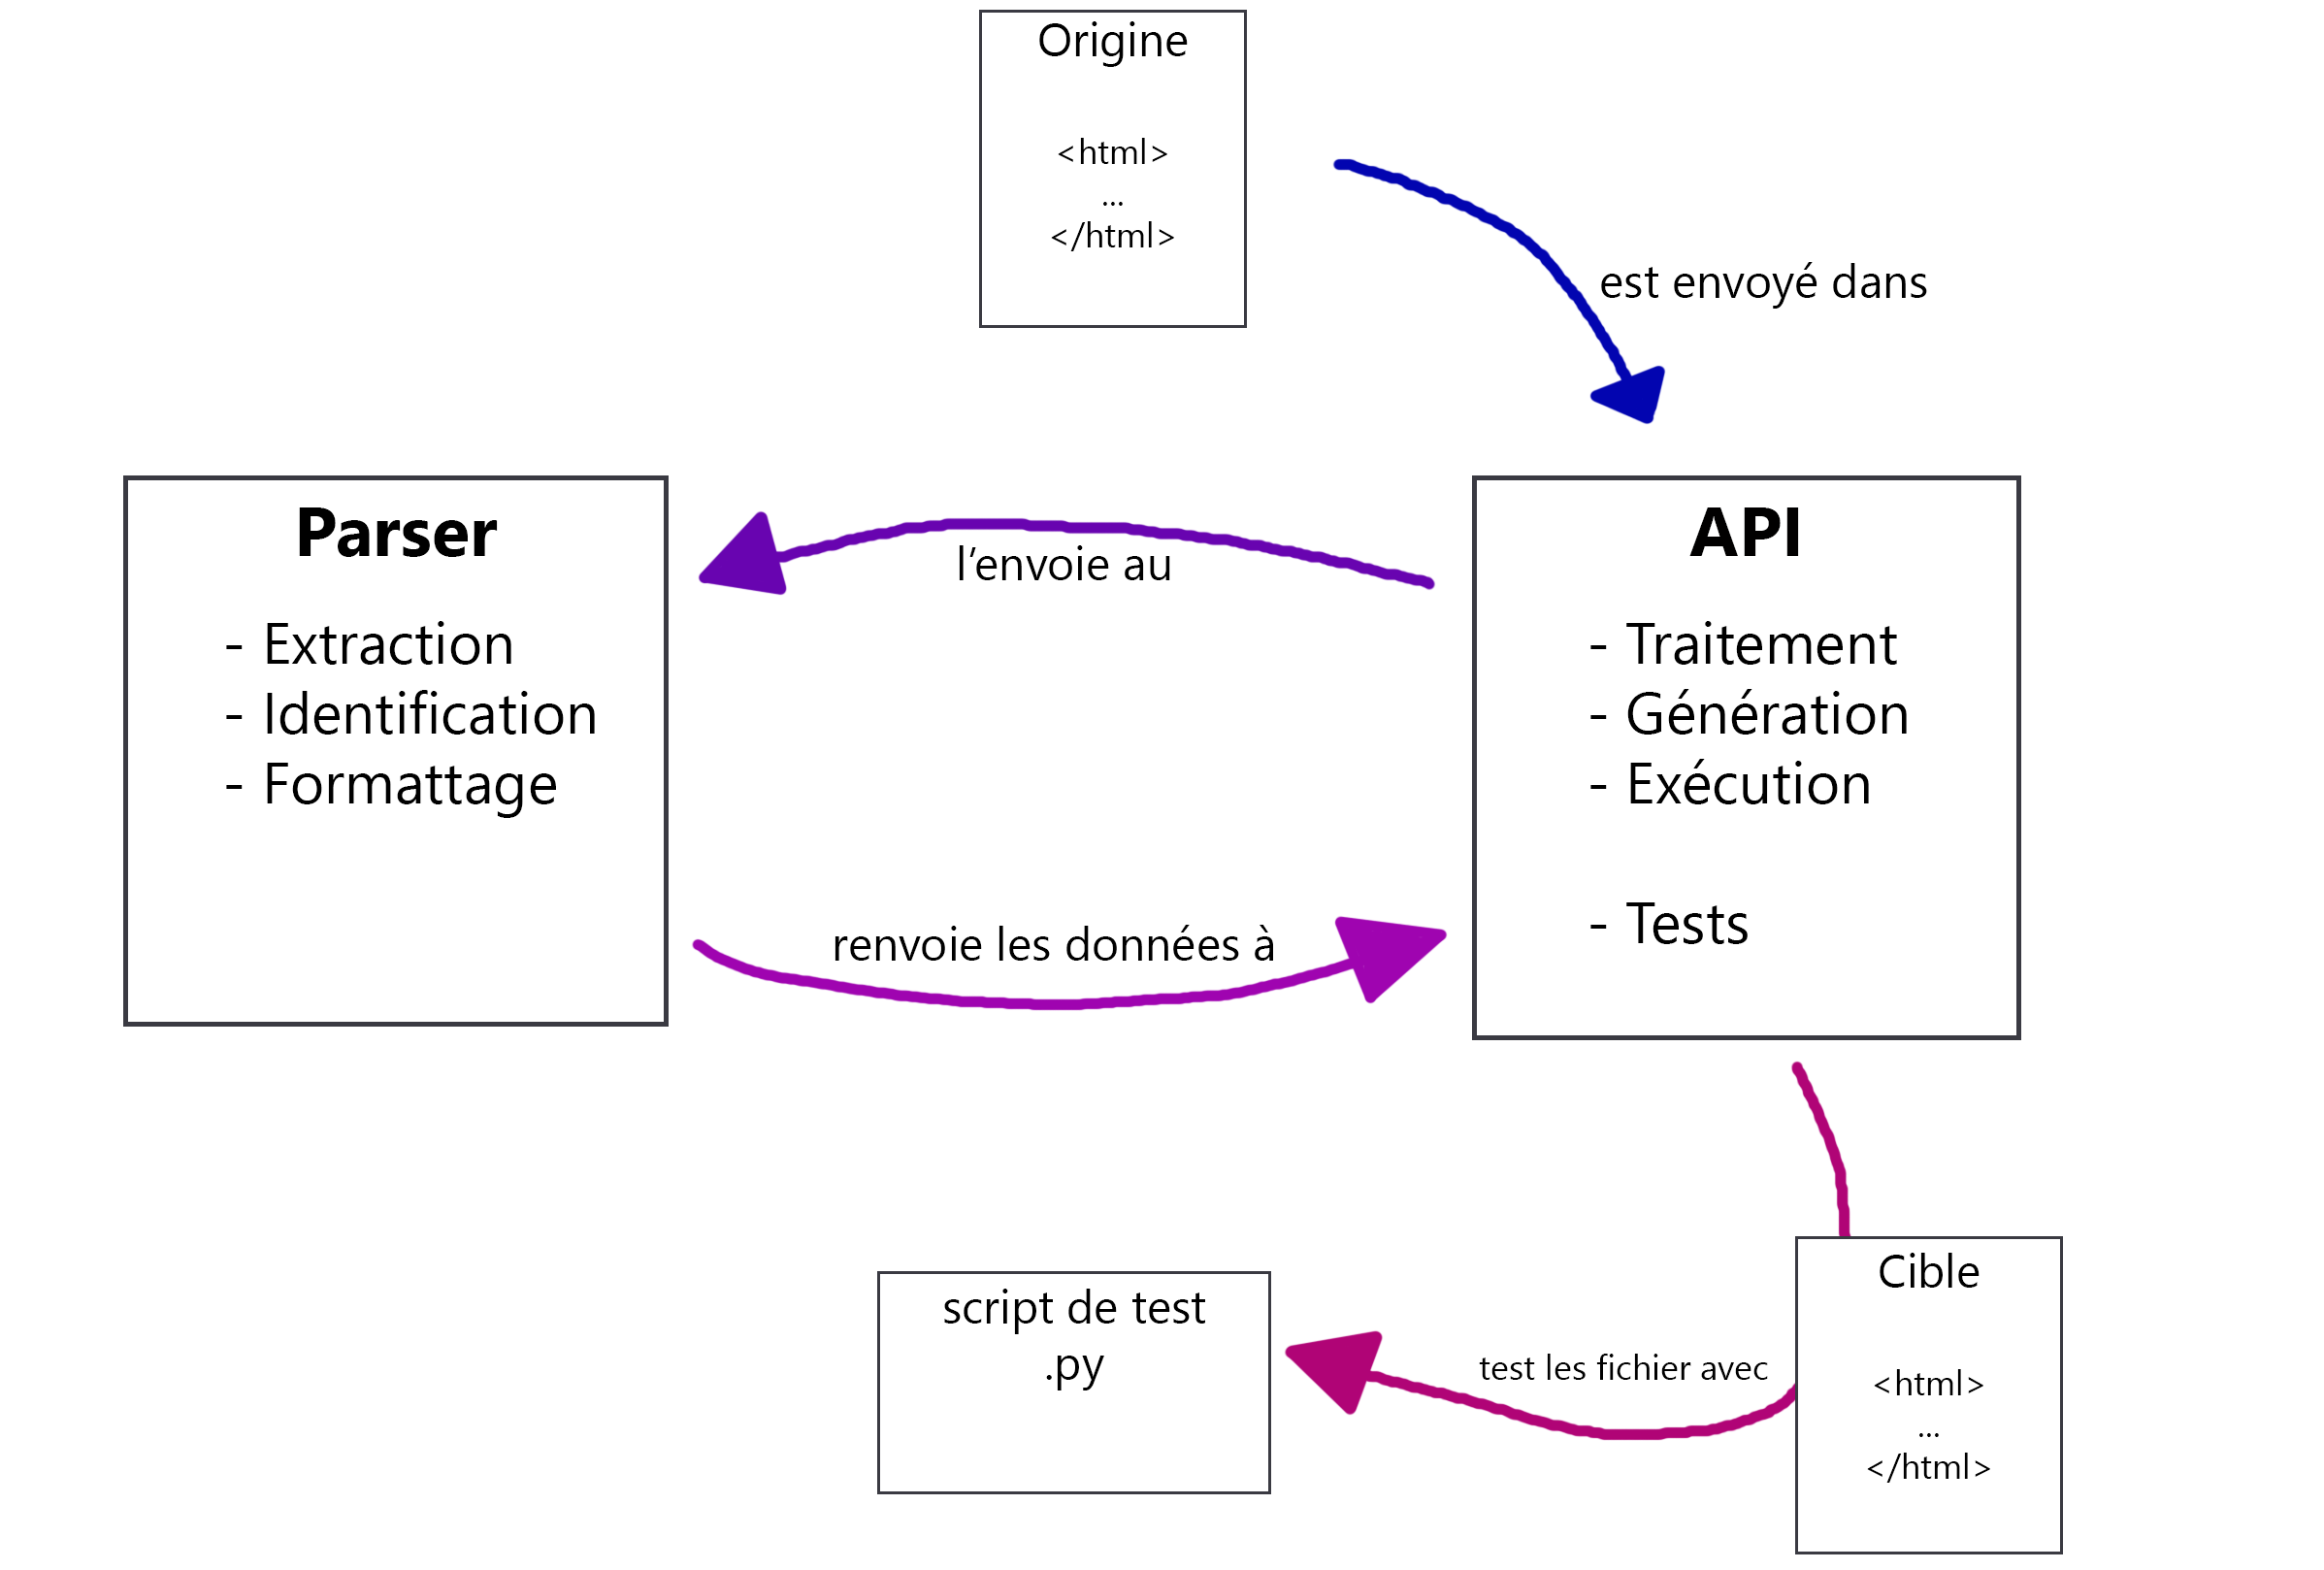
\includegraphics[width=1\textwidth]{schema.png}
\caption{\label{fig:schema}Schéma de l'API, du parser et de leur intéraction avec les autres éléments}
\end{figure}

C'est cette logique que je suivrais de manière constante sur tout le long de la mission quand il s'agira de passer à l'objectif SQL et PHP. toot\\

Après un premier travail d'intégration, cette logique n'est pas entièrement intégrable dans la plate-forme. La plate-forme ne peut pas garder un fichier de script dont l'exécution permet de tester les fichiers "cible". Cependant, le script en lui-même peut être garder en mémoire afin d'être exécuter plus tard. L'intégration n'étant pas au cœur de la mission à l'instant présent, ce travail peut attendre d'être effectué plus tard dans le courant de sa réalisation.\\

\section{Réalisation}

Je vais dans cette partie élaborer le procédé que j'ai suivis afin de mettre au point l'API, la logique que j'ai suivi et les choix que j'ai fait dans la structuration de l'API.\\

\subsection{Le Parser}

Le parser agit comme l’interpréteur de l'API. L'API envoie le contenu HTML qu'elle récupère dans un fichier et le parser lui renvoie de manière formater les données qu'il l'intéresse.\\

Basé sur HTMLParser, il hérite de trois fonctions qui lui permet de réagir lorsqu'il rencontre une balise entrante, une balise sortante et du contenu. Une fois l'un de ses trois, il enregistre les balises dans un certain format dans une liste, et, à l'aide d'autres fonctions, renvoie les données enregistrées sous forme de liste à l'API.\\

Après plusieurs réécritures du format des données, sa dernière version formate les informations de la manière suivante : type-balise\#id pour déterminer l'ouverture ou la fermeture d'une balise, balise\#id-content pour le contenu d'une balise et attribut\#id-content pour l'attribut d'une balise.\\

Ces données sous format STRING sont stockées dans des listes de STRING, une pour les balises, une pour les contenu et une pour les attributs.\\

\begin{figure}[ht]
\centering
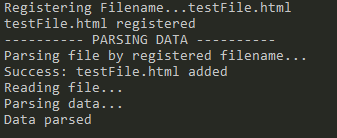
\includegraphics[width=1\textwidth]{parsing.png}
\caption{\label{fig:parsing}Résultat de l'extraction des données sur un fichier "origine" ou "cible"}
\end{figure}

\subsection{Génération des tests}

Une fois les données récupérées, l'API va pouvoir commencer son analyse. En parcourant les listes renvoyées par le parser, il identifie les points à tester comme par exemple le contenu d'une balise "P" ou les attributs "ID" des balises présentes dans le fichier. Après cette analyse, il écrit un script qui va renvoyer les données qui vont lui permettre de comparer la validité d'un fichier "cible", comme le contenu de la balise "TITRE" ou "P", ainsi que les tests à effectuer sur le fichier "cible".\\

À chaque exécution de test, un message est envoyé dans le log pour dire si le test est passé en renvoyant un booléen qui permet de suivre l'ordre d'exécution des tests.\\

\subsection{Exécution des tests}

À l'exécution de ce script, l'API va encore une fois faire appel au parser afin d'extraire le contenu du fichier "cible". Il va effectuer une première série de test sur ce fichier en testant la validité du fichier en lui-même. Il vérifie entre autre sur il n'y a pas d'erreur dans l'ouverture et la fermeture des balises ou encore si le header se trouve avant le body. Il lit aussi si des données appartiennent à la même balise afin de vérifier si il s'agit d'un ajout libre de la part de l'auteur du fichier "cible" ou si le fichier "origine" contient une balise qui aurait plusieurs propriétés et d'effectuer des tests supplémentaires dessus. J'appelle cette catégorie de test les tests "primaires", ou "indispensables".\\

Ensuite, on effectue une deuxième série de test sur le fichier. Ces tests correspond aux tests qui vise des balises en particulier et qui ne s'effectue que dans le cas où la balise est présente dans le fichier. Si il y a une balise "IMG", vérifié la présence d'un attribut "SRC", que cette attribut soit de préférence défini avec un chemin relatif plutôt qu'un chemin absolue, et bien évidemment si cette balise est définie dans le fichier "origine" que ce chemin corresponde bien au chemin indiqué dans le fichier "origine". J'appelle cette catégorie de test les tests "secondaires".\\

\begin{figure}[ht]
\centering
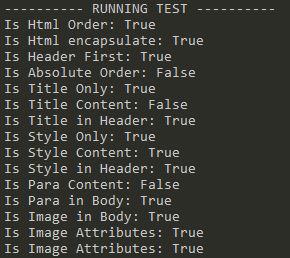
\includegraphics[height=0.63\textwidth]{running.png}
\caption{\label{fig:running}Exécution des tests sur un fichier "cible"}
\end{figure}

\subsection{Résultats des tests}

Une fois les tests exécutés, l'API renvoie un log des tests passées et des tests ratés sous la forme de texte. Dans ce log est d'abord présenté le nombre de tests "primaire" et "secondaire" passés par rapport au nombre totale respectif de tests effectués sur le fichier. Est ensuite décrit les tests échoués avec une description de ce qui a été échoué.\\

\begin{figure}[ht]
\centering
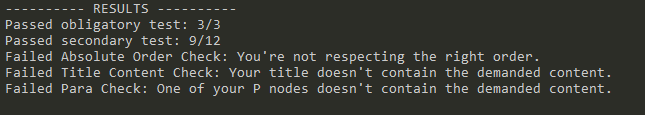
\includegraphics[width=1\textwidth]{results.png}
\caption{\label{fig:results}Script Python généré suite à l'analyse d'un fichier "origine"}
\end{figure}

\section{Déroulement}

Ce stage s'est donc divisé en trois étapes :\\

\subsection{Expérimentation}

La première partie a été l'apprentissage des outils utilisés dans l'API. Bien que j'étais familier avec le Python, il a fallu une période de réapprentissage pour réapprendre certaines fonctionnalités du langage n'y ayant pas retouché sur une grande période de temps. Il a fallu aussi prendre en main HTMLParser, et se renseigner sur le fonctionnement des différentes méthodes fournies par la librairie.\\

Pour apprendre, j'ai utilisé un fichier HTML relativement simple utilisant quelques balises. J'ai utilisé trois des méthodes proposés :\\

\begin{enumerate}
\item handle\_starttag
\item handle\_endtag
\item handle\_data
\end{enumerate}

La première fonction, à la rencontre d'une balise ouvrant va enregistrer la balise sous la forme d'un dictionnaire de données avec les attributs et autres propriétés. La deuxième fonctionne dans le même principe mais agit lorsqu'elle rencontre une balise fermante.\\

La troisième agit lorsqu'elle rencontre du contenu. La raison pour laquelle il est important de définir cette méthode correctement est parce que le contenu n'est pas définit selon la balise, mais selon les caractères qu'elle rencontre. Si par exemple après l'ouverture d'une balise "BODY" on fait un retour à la ligne, ou "\textbackslash n", la méthode détecte le retour à la ligne comme étant du contenu. Dés le début j'y ai remédié simplement en enregistrant la balise entrante dans laquelle le curseur qui parcoure l'HTML se trouve, et selon la balise dans laquelle il se trouve, enregistré le contenu rencontré.\\

J'ai ensuite continué en testant directement certaines balises et certaines propriétés de ces balises. J'ai réalisé un test sur la balise "HTML" qui encapsule tout le contenu HTML ("HEADER", "BODY") ainsi que la position de la balise "TITRE" dans le "HEADER" afin d'avoir une base sur laquelle continué lors du développement de l'API.\\

\subsection{Développement}

Le parser étant maintenant opérationnel, j'ai put commencer sur la partie fonctionnelle de l'API : la génération des tests, des tests rudimentaires ayant été déjà créé afin de pouvoir tester la génération et l'exécution des tests à partir d'un fichier "origine" sur un fichier "cible". L'identification des balises à tester se fait en parcourant les balises découvertes en activant les tests correspondant par le biais d'un booléen. Une fois l'identification réalisée, la génération des tests parcourent ces booléens et génèrent le script qui va jouer sur les fichiers "cible".\\

\begin{figure}[ht]
\centering
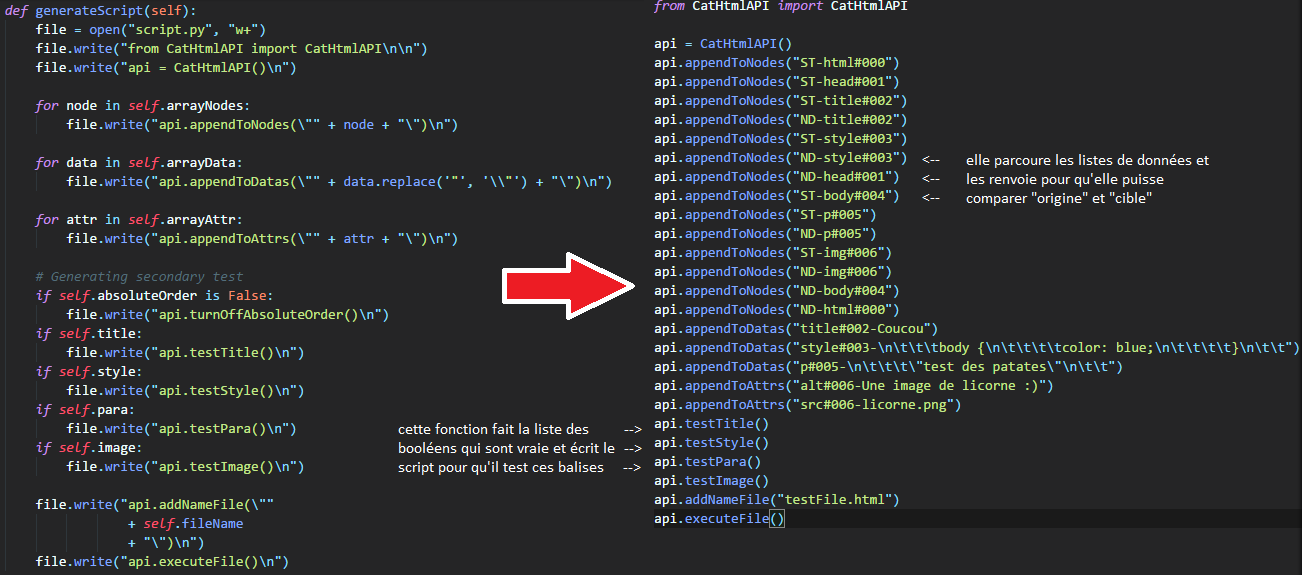
\includegraphics[width=1\textwidth]{scripts-envoye.png}
\caption{\label{fig:scriptenv}Résultat des tests sur un fichier "cible"}
\end{figure}

À partir de ce patron, j'ai continué à identifier les autres balises et à extraire leurs contenus de la même façon. Il a fallu prendre du recul à chaque écriture de tests que ce soit des test "primaire" ou "secondaire" dû à l'intérêt principale de l'outil que je suis en train de développer pour C.A.T. En effet, ce sont des tests visant à la vérification de fichier appartenant à des personnes cherchant à apprendre l'HTML, le SQL et le PHP. Il faut donc s'abstraire de ce que l'on considère comme acquis.\\

Il faut alors analyser les étapes par lesquelles on passe lorsque l'on écrit un élément et ce qui le compose.\\

Par exemple, j'écris un titre dans ma page HTML. Je vais donc pour cela le mettre dans une balise "TITRE". Cependant, il y a plus d'étape que ça lors de la création d'une balise "TITRE". Il faut écrire la balise "TITRE" dans le HEADER et il ne peut y avoir que une seule balise "TITRE". De même, il faut aussi qu'il y ait obligatoirement au moins une balise "TITRE" dans le document.\\

Afin d'extraire les les données pour les tester et les comparer, j'utilisais d'abord du "slicing" sur les STRING de données afin de récupérer les parties qui m'intéressait. Sur un exemple de contenu, "title-Mon Titre", je faisais donc exemple[:5] afin de récupérer les 5 premiers caractères, donc "titre" pour identifier la balise sur laquelle je récupérais le contenu et exemple[6:] pour exclure les 6 premiers caractères "titre-" pour le contenu de la balise. Très vite cette méthode s'est avérée inconsistante lorsqu'il a fallu intégrer d'autres éléments à la chaîne de caractères et surtout dans le cas où il fallait identifier d'autres balises qui n'ont pas le même nombre de caractères dans leurs noms, comme la balise "P". Le "slicing" prête à confusion puisqu'il est moins explicite. J'ai rencontré des problèmes en l'utilisant ne serait-ce que quand j'ai changé la définition d'un caractère dans la chaîne, que les tests s'affichaient comme tant échoué car il ne réussissait pas à capturer la bonne partie de la chaîne de caractère. À ce moment, j'ai arrêté d'utiliser le "slicing" et suis passé à l'utilisation de la fonction split qui coupe la chaîne de caractère à partir d'un caractère pré-défini.\\

\subsection{Approfondir}

Une fois la première étape de développement de l'API faites, il a fallu approfondir la boite a outils de l'API. À ce stade, l'API exécute les tests de manières primitives. On s'est mis dans la peau d'un utilisateur qui n'en faisait ni moins ni plus. Un utilisateur standard qui respecte les règles sans pour autant être insensible a l'erreur. Il faut maintenant imaginer le scénario d'utilisateur qui ne sait pas ce qu'il fait quand il répond à des questions ou essaye de combler les trous à l'aide de bouts de code trouvés en ligne qui peut contenir du faux ainsi que des informations supplémentaires et/ou optionnelles.\\

Cette fois-ci, de nouveaux tests à réaliser comme vérifier que le HEADER se place bien avant le BODY mais surtout que le contenu demandé soit présent avec les propriétés demandées.\\

Nous voyons ici trois scénario possible :\\

\begin{enumerate}
\item "origine" demande simple une balise "P" avec un paragraphe dedans, "cible" avec une balise "P" et un paragraphe dedans
\item "origine" demande simple une balise "P" avec un paragraphe dedans, "cible" avec une balise "P", un paragraphe dedans et des attributs supplémentaires
\item "origine" demande simple une balise "P" avec un paragraphe dedans des attributs supplémentaires, "cible" avec une balise "P", un paragraphe dedans et des attributs supplémentaires\\
\end{enumerate}

Pour ces trois cas, il faut donc lier les éléments ensemble et pouvoir vérifier le contenu "origine" et s'assurer qu'il y a un contenu "cible" qui correspond et fait le minimum que ce que "origine" fait.\\

Cela implique d'abord lors de l'extraction des données dans le parser que les éléments soit liés ensemble ce qui a amené un changement dans le format et à un ajout de fonctionnalités au parser. Ce changement de format inclus dorénavant une clé qui permet de lier les éléments entre eux. Prenons par exemple une balise "P" avec un paragraphe "Paragraphe" et un attribut "ID" d'une valeur de "152". Maintenant, on lit les chaînes ainsi :\\

\begin{enumerate}
\item "ST-p\#005", pour l'ouverture de "P"
\item "ND-p\#005", pour la fermeture de "P"
\item "p\#005-Paragraphe", pour le contenu de "P"
\item "id\#005-152", pour l'attribut "ID" de "P"\\
\end{enumerate}

Cette clé rajoutée sur dans les chaînes est calcule de manière simple en s’incrémente a chaque fois qu'il finit de générer une balise entrante. Elle apparaît sous la forme de trois caractères allant de 000 à 999, laissant 1000 possibilités d'ouverture de balises. Bien que pas nécessaire en pratique, puisque la balise fermante n'a jamais vu le besoin d’être testé, j'ai tout de même décidé de rajouter la clé a la balise fermante en suivant l’idée qu'il ne faut pas se dire que ça ne devrait pas arriver, ou que cela ne semble pas possible, les utilisateurs trouveront un moyen pour qu'ils faillent corriger la faute. Le procédé pour récupérer la clé pour une balise fermante est plus compliqué cependant. La variable compteur qui agit en clé n'est pas utilisable car il est toujours possible d’être dans un labyrinthe de balise. À la place, je remonte la liste de balise rencontré en vérifiant trois possibilités :\\

\begin{enumerate}
\item en troisième, si il rencontre une balise fermante in incrémente une variable
\item en deuxième, si il rencontre une balise fermante il décrémente la variable
\item en premier, si la balise rencontré est une balise entrante de même nom que celle qui se ferme et que la variable est à zéro, il récupère l'id et se l'approprie\\
\end{enumerate}

Ce changement au parser a mené à un changement dans l'API puisque maintenant le format des string étudiés dans l'API pour les tests est différent et a lancé une nouvelle refonte de l'API dans l'analyse des données ainsi que dans les tests.\\